\documentclass[a4paper, 12pt]{article}		% general format

%%%% Charset
\usepackage{cmap}							% make PDF files searchable and copyable
\usepackage[utf8x]{inputenc}				% accept different input encodings
\usepackage[T2A]{fontenc}					% Russian font
\usepackage[russian]{babel}					% multilingual support (T2A)

%%%% Graphics
\usepackage[dvipsnames]{xcolor}			% driver-independent color extensions
\usepackage{graphicx}						% enhanced support for graphics
\usepackage{wrapfig}						% produces figures which text can flow around

%%%% Math
\usepackage{amsmath}						% American Mathematical Society (AMS) math facilities
\usepackage{amsfonts}						% fonts from the AMS
\usepackage{amssymb}						% additional math symbols

%%%% Typography (don't forget about cm-super)
\usepackage{microtype}						% subliminal refinements towards typographical perfection
\linespread{1.3}							% line spacing
\usepackage[left=2.5cm, right=1.5cm, top=2.5cm, bottom=2.5cm]{geometry}
\setlength{\parindent}{0pt}					% we don't want any paragraph indentation
\usepackage{parskip}						% add distance between paragraphs

%%%% Tables
\usepackage{tabularx}						% Normal tables
\usepackage{multirow}						% for tabular
\usepackage{hhline}							% for tabular


%%%% Other
\usepackage{url}							% verbatim with URL-sensitive line breaks
\usepackage{fancyvrb}						% verbatim with box
\setcounter{secnumdepth}{5}					%

%------------------------------------------------------------------------------
\usepackage{listings}						% typeset source code listings

% Настройки отображения кода
\lstset{
	% Настройки отображения
	breaklines=true,						% Перенос длинных строк
	basicstyle=\ttfamily\footnotesize,		% Шрифт для отображения кода
	frame=tblr								% draw a frame at all sides of the code block
	tabsize=2,								% tab space width
	showstringspaces=false,					% don't mark spaces in strings
	% Настройка отображения номеров строк. Если не нужно, то удалите весь блок
	numbers=left,							% Слева отображаются номера строк
	stepnumber=1,							% Каждую строку нумеровать
	numbersep=5pt,							% Отступ от кода
	numberstyle=\small\color{black},		% Стиль написания номеров строк
}

% Для настройки заголовка кода
\usepackage{caption}
\renewcommand{\lstlistingname}{Листинг} % Переименование Listings в нужное именование структуры
%------------------------------------------------------------------------------

\begin{document}

\begin{titlepage}
\thispagestyle{empty}

\begin{center}
Санкт-Петербургский политехнический университет Петра Великого\\
Институт Информационных Технологий и Управления\\*
Кафедра компьютерных систем и программных технологий\\*
\hrulefill
\end{center}

\vspace{15em}

\begin{center}
\textsc{\textbf{Научно-исследовательская работа}}
\vspace{1em}

%Дисциплина: \textbf{Методы оптимизации}
\vspace{2em}

Тема: \textbf{Установка WSO2 Enterprise Mobility Manager}
\end{center}

\vspace{16em}

\begin{flushleft}
Выполнил студент гр. 53501/3 \hrulefill С.А. Мартынов \\
\vspace{1.5em}
Руководитель, к.т.н.,доц. \hrulefill И.В. Стручков\\
\end{flushleft}

\vspace{\fill}

\begin{center}
Санкт-Петербург \\
2015
\end{center}

\end{titlepage}
\setcounter{page}{2}

\tableofcontents{}
\newpage
%------------------------------------------------------------------------------

\section*{Введение}
\addcontentsline{toc}{section}{Введение}

Компания WSO2 разрабатывает ряд продуктов на общей платформе Carbon и собственную среду разработки -- WSO2 Developer Studio.

\section{WSO2 Enterprise Service Bus}

Enterprise Service Bus обеспечит интеграцию с корпоративными сервисами.

Сервисная шина, это связующее программное обеспечение, обеспечивающее централизованный и унифицированный событийно-ориентированный обмен сообщениями между различными информационными системами на принципах сервис-ориентированной архитектуры. Основной принцип сервисной шины -- концентрация обмена сообщениями между различными системами через единую службу, в которой, при необходимости, обеспечивается транзакционный контроль, преобразование данных, сохранность сообщений. Все настройки обработки и передачи сообщений предполагаются также сконцентрированными в едином сервисе, и формируются в терминах служб, таким образом, при замене какой-либо информационной системы, подключённой к шине, нет необходимости в перенастройке остальных систем.

У ESB может быть множество применений. С ее помощью можно организовать взаимодействие между системами, которые до этого не были приспособлены для обмена между собой (например шлюз между протоколами REST и SOAP). Сервисная шина предприятия может производить агрегацию данных "на-лету" из множества источников и предоставление их в виде унифицированного сервиса. Шина также может выступать как интеллектуальный балансировщик нагрузки и маршрутизатор сообщений уровня приложений.

Ключевые возможности
\begin{itemize}
\item Обработка и преобразование сообщений.
\item Статическая и алгоритмическая маршрутизация сообщений.
\item Доступ к данным из сторонних информационных систем с помощью готовых или специально разработанных адаптеров.
\item Использование защищённого транспорта, с гарантированной доставкой сообщений, поддерживающего транзакционную модель.
\end{itemize}

\section{WSO2 Enterprise Mobility Manager}

\subsection{Требования к ПО}

От хоста, на котором будет запускаться Enterprise Mobility Manager требуется иметь минимум 2 ГБ свободной оперативной памяти (512 МБ будут использованы для SOAP-сообщений, что достаточно для не большого количество пользователей но может создать проблемы при использовании в производственной среде). На винчестере потребуется порядка 1 Гб, на считая места, которое потребуется для хранения баз данных и лог-файлов.

Все продукты WSO2 на платформе Carbon запускаются и нормально работают на Oracle JDK 1.6.*/1.7.*. Версия JDK 1.8 на данный момент не поддерживается. Также разработчики не рекомендуют использовать OpenJDK.

В качестве базы данных можно использовать встроенное решение H2, которое обеспечивает потребности разработчиков и тестировщиков, но для развёртывания в реальной среде строит использовать полноценные СУБД -- Oracle, PostgreSQL, MySQL, MS SQL и т.д.

Для интеграции с существующей базой пользователей, поддерживается интеграция с OpenLDAP.

На клиентах (мобильных устройствах) на данный момент поддерживаются версии 6.0 - 7.0 для iOS, для Android:
\begin{itemize}
\item Ice Cream Sandwich (4.0.3 – 4.0.4)
\item Jelly Bean (4.1 – 4.3.1)
\item KitKat (4.4 – 4.4.4)
\item Lollipop (5.0)
\end{itemize}

Общий список программного обеспечения, которое может потребоваться, выглядят следующим образом:

\begin{tabular}{|c|c|c|}
\hline 
ПО & Версия & Примечание \\ 
\hline 
{Oracle JDK} & 1.6.24 или новее / 1.7 & Для запуска приложения \\ 
\hline 
MySQL & 5.6.* & База данных \\ 
\hline 
MySQL Connector/J & 5.1.* & Используется для связи с БД \\ 
\hline 
Git & 1.8.* & Для доступа к репозиторию Android Agent \\ 
\hline 
Eclipse & Juno (4.2.1) или новее & Сборка клиентских приложений \\ 
\hline 
Android SDK & Уровень 8 - 17 & Сборка клиентских приложений \\ 
\hline 
Web-браузер & * & Для доступа к веб-интерфейсу \\ 
\hline 
Apache Ant & 1.7.0 или новее & Компиляция и сборка примеров приложений \\ 
\hline 
Apache Maven & 3.0.* & Сборка приложения из исходных кодов \\ 
\hline 
\end{tabular} 

\subsection{Подготовка хоста}

\subsubsection{Oracle JDK}

На основании предыдущего пункта, необходимо установить JDK1.7. Все действия будем проводить на Ubuntu 15.04 Server.

\begin{Verbatim}[frame=single]
user@wso2:~ cat /etc/lsb-release 
DISTRIB_ID=Ubuntu
DISTRIB_RELEASE=15.04
DISTRIB_CODENAME=vivid
DISTRIB_DESCRIPTION="Ubuntu 15.04"
\end{Verbatim}

Установку Java можно провести вручную, скачав исходники с сайта Oracle, но мы воспользуемся PPA, в котором эта процедура автоматизированная.

Для начала убедимся, что у нас уже не установлен OpenJDK.

\begin{Verbatim}[frame=single]
user@wso2:~ java -version
The program 'java' can be found in the following packages:
 * default-jre
 * gcj-4.9-jre-headless
 * openjdk-7-jre-headless
 * gcj-4.8-jre-headless
 * openjdk-6-jre-headless
 * openjdk-8-jre-headless
Try: sudo apt-get install <selected package>
\end{Verbatim}

Как видно выше, система ничего не знает о Java, значит можно продолжить выполнение установки. В противном случае потребовалось бы очистить систему от имеющихся пакетов командой (на самом деле в системе допустимо иметь несколько различных версий JDK и переключаться между ними, но мы сейчас это рассматривать не будем).
\begin{Verbatim}[frame=single]
sudo apt-get remove openjdk*
\end{Verbatim}

Теперь можно перейти к добавлению PPA, содержащего JDK1.7. Для этого потребуется ввести следующие три команды (использование sudo требует ввода пароля суперпользователя).
\begin{Verbatim}[frame=single]
echo "deb http://ppa.launchpad.net/webupd8team/java/ubuntu vivid main" |\
                   sudo tee /etc/apt/sources.list.d/webupd8team-java.list
echo "deb-src http://ppa.launchpad.net/webupd8team/java/ubuntu vivid main" |\
                sudo tee -a /etc/apt/sources.list.d/webupd8team-java.list
sudo apt-key adv --keyserver hkp://keyserver.ubuntu.com:80\
                                                       --recv-keys EEA14886
\end{Verbatim}

Обновление списка пакетов и установка JDK.

\begin{Verbatim}[frame=single]
sudo apt-get update
sudo apt-get install oracle-java7-installer oracle-java7-set-default
\end{Verbatim}

В процессе установки потребуется принять лицензию Oracle.

После установки стоит убедиться в корректности работы JDK и наличию всех необходимых переменных окружения (для этого нужно завершить текущий сеанс и залогиниться по новой)

\begin{Verbatim}[frame=single]
user@wso2:~ java -version
java version "1.7.0_80"
Java(TM) SE Runtime Environment (build 1.7.0_80-b15)
Java HotSpot(TM) 64-Bit Server VM (build 24.80-b11, mixed mode)
user@wso2:~ javac -version
javac 1.7.0_80
user@wso2:~ env | grep -i java
DERBY_HOME=/usr/lib/jvm/java-7-oracle/db
PATH=/usr/local/sbin:/usr/local/bin:/usr/sbin:/usr/bin:/sbin:/bin:/usr/games:
/usr/local/games:/usr/lib/jvm/java-7-oracle/bin:/usr/lib/jvm/java-7-oracle/db
/bin:/usr/lib/jvm/java-7-oracle/jre/bin
JAVA_HOME=/usr/lib/jvm/java-7-oracle
J2SDKDIR=/usr/lib/jvm/java-7-oracle
J2REDIR=/usr/lib/jvm/java-7-oracle/jre
\end{Verbatim}

\subsubsection{MySQL сервер}

Теперь нужно установить сервер баз данных. Используем для этого MySQL.

\begin{Verbatim}[frame=single]
sudo apt-get install mysql-server mysql-client
\end{Verbatim}

В процессе установки потребуется указать пароль для администратора баз данных.

Далее нужно запустить сервер и произвести подключение, используя пароль администратора.

\begin{Verbatim}[frame=single]
sudo /etc/init.d/mysql start 
mysql -u root -p
\end{Verbatim}

В консоли базы данных, нужно создать новую БД и пользователя для этой базы (zz11aa22 -- пароль пользователя).

\begin{Verbatim}[frame=single]
create database EMM_DB;
GRANT ALL ON EMM_DB.* TO admin@localhost IDENTIFIED BY "zz11aa22";
\end{Verbatim}

\subsubsection{Enterprise Mobility Manager}

WSO2 Enterprise Mobility Manager можно собрать из исходников либо воспользоваться готовыми бинарниками, распространяемыми разработчиками (размер архива 277MB).

\begin{Verbatim}[frame=single]
user@wso2:~ wget http://product-dist.wso2.com/products/enterprise-mobility-ma
nager/1.1.0/wso2emm-1.1.0.zip
\end{Verbatim}

Содержимое архива нужно извлечь в директорию на винчестере, я предпочитаю для этого использовать opt.

\begin{Verbatim}[frame=single]
sudo unzip wso2emm-1.1.0.zip -d /opt
\end{Verbatim}

\subsubsection{Взаимодействие с БД}

Скрипт со структурой базы данных находится в папке с EMM. Требуется ввести пароль, который был задан для пользователя admin (zz11aa22).

\begin{Verbatim}[frame=single]
mysql -u admin -p -DEMM_DB < /opt/wso2emm-1.1.0/dbscripts/mysql.sql
\end{Verbatim}

Взаимодействие Java и MySQL обеспечивает mysql-connector-java. 

\begin{Verbatim}[frame=single]
sudo apt-get install libmysql-java
\end{Verbatim}

Далее нужно указать программе, что информацию можно получать из MySQL. Для этого нужно отредактировать файл /opt/wso2emm-1.1.0/repository/conf/datasources/master-datasources.xml.

\begin{itemize}
\item Поле <url> -- \url{jdbc:mysql://localhost:3306/EMM_DB}
\item Поле <username> -- admin
\item Поле <password> -- zz11aa22
\item Поле <driverClassName> -- com.mysql.jdbc.Driver
\end{itemize}

\subsubsection{Настройка почтовых уведомлений}

В директории \url{/opt/wso2emm-1.1.0/repository/deployment/server/jaggeryapps/mdm/config/} нужно создать файл config.json, пользуясь шаблонами из директории \url{/opt/wso2emm-1.1.0/repository/deployment/server/jaggeryapps/mdm/config/tempConfigs/}.

Скопировать файлы config.json и ui.json из \url{/opt/wso2emm-1.1.0/repository/deployment/server/jaggeryapps/mam/config/tempConfigs/} в \url{/opt/wso2emm-1.1.0/repository/deployment/server/jaggeryapps/mam/config/} и изменить настройки работы с почтовым сервером.

В директории \url{/opt/wso2emm-1.1.0/repository/deployment/server/jaggeryapps/publisher/config/} файл mam-config.json.temp переименовать в mam-config.json.

\subsubsection{Определение имени сервера}

В файле \url{/opt/wso2emm-1.1.0/repository/conf/carbon.xml} указывается доменное имя сервера. Не имея имени, можно указать IP-адрес.

\begin{Verbatim}[frame=single]
<HostName>192.168.124.169</HostName>
<MgtHostName>192.168.124.169</MgtHostName>
\end{Verbatim}

\subsection{Запуск Enterprsie Mobility Manager}

\subsubsection{Ручной запуск EMM}

Для запуска воспользуемся скриптом из архива. Пока сделаем это от имени суперпользователя, позже разберёмся с правами более тонко.
\begin{Verbatim}[frame=single]
sudo -E sh /opt/wso2emm-1.1.0/bin/wso2server.sh
\end{Verbatim}

Когда система будет запущена, из браузера можно будет обратиться по адресу \url{https://192.168.124.185:9443/} (192.168.124.185 - мой IP виртуальной машины с WSO2 Enterprsie Mobility Manager) и получить доступ к панели управления (рисунок 1). Имя пользователя и пароль по умолчанию admin.

\begin{figure}[h!]
\centering
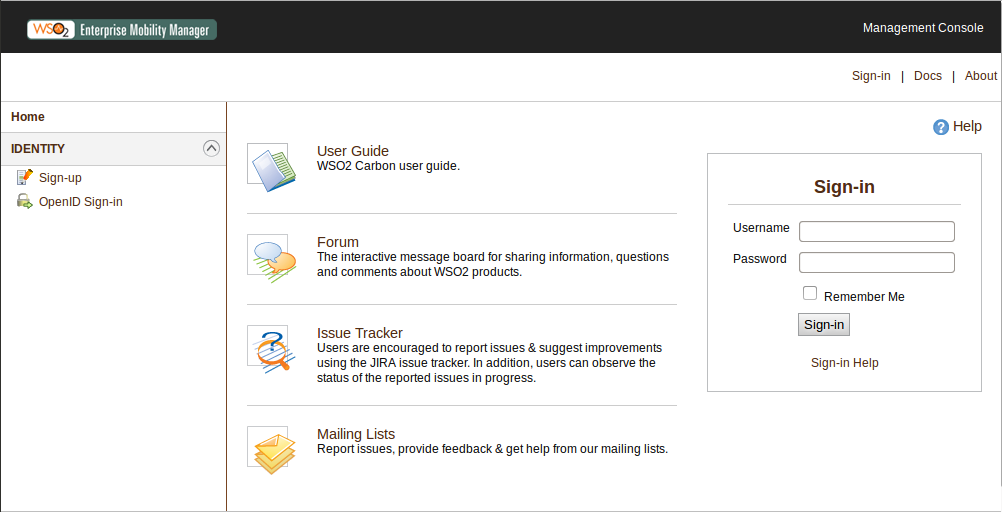
\includegraphics[scale=0.45]{res/EMM001}
\caption{Web-интерфейс EMM}
\end{figure}

\subsubsection{Автоматический запуск EMM}

В предыдущем пункте мы рассмотрели ручной запуск приложения. Это удобно для разработки и отладки, но на реальном сервере требуется запуск в качестве сервиса. Для этого можно использовать следующий скрипт (листинг 1).

Этот скрипт будет работать с системой upstart. Для этого его нужно сохранить в директорию /etc/init.d/ и обновить кэш скриптов.

\begin{Verbatim}[frame=single]
sudo update-rc.d appserver defaults
\end{Verbatim}

После этого можно запускать приложение привычным образом.

\begin{Verbatim}[frame=single]
service WSO2EMM {start|stop|restart}
\end{Verbatim}

В связи с переходом Ubuntu и многих других ведущих дистрибутивов на работу с systemd, скрипт нужно будет переписать на работу с новой системой инициализации.

\lstinputlisting[language={bash},caption={Скрипт WSO2EMM.sh}]{res/WSO2EMM.sh}

\subsection{Добавление устройств}

Для управления мобильными устройствами нужно перейти по адресу \url{https://192.168.124.185:9443/sso/login}, имя пользователя и пароль -- admin.

\begin{figure}[h!]
\centering
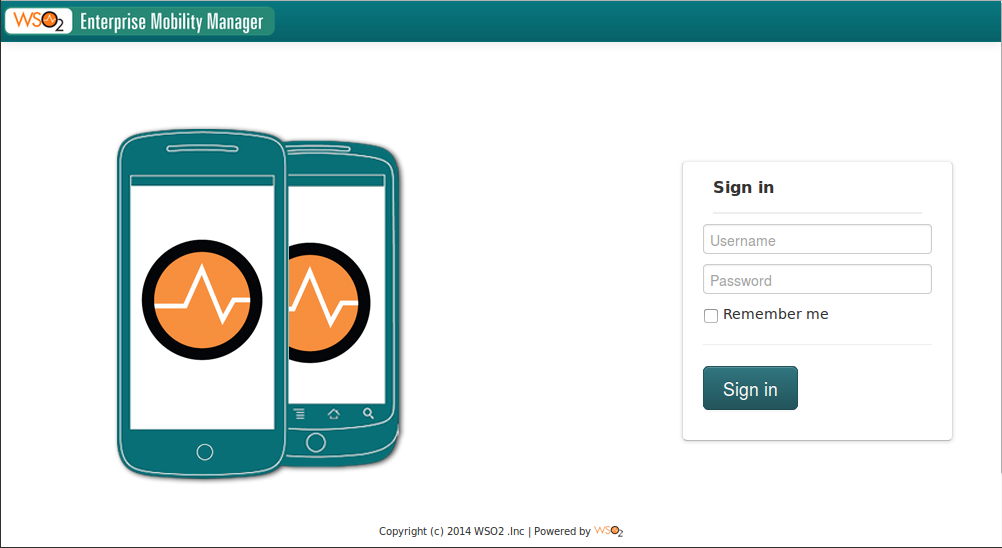
\includegraphics[scale=0.45]{res/EMM002}
\caption{Управление мобильными устройствами}
\end{figure}

\subsubsection{Настройка клиента}

Система работает по принципу приглашений -- администратор создаёт пользователя, определяет его уровень полномочий и высылает приглашение на его e-mail. Пароль пользователя генерируется автоматически и приходит пользователю в письме вместе со ссылкой на скачивание приложения.

\begin{figure}[h!]
\centering
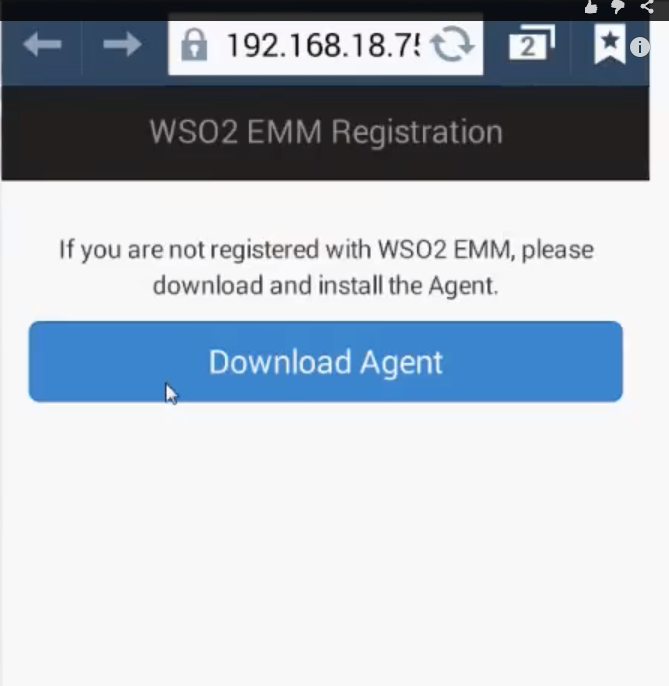
\includegraphics[scale=0.45]{res/EMM003}
\caption{Установка агента}
\end{figure}

В процессе установки мобильного клиента, у пользователя выясняется, является ли устройство его собственностью, или принадлежит фирме (см. рис. 4). В зависимости от этого определяются права администратора. В моём случае администратор получал полные права вне зависимости от выбора пользователя.

\begin{figure}[h!]
\centering
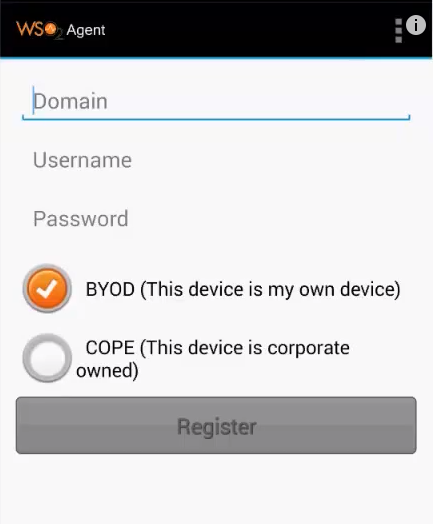
\includegraphics[scale=0.65]{res/EMM004}
\caption{Определение прав администратора}
\end{figure}

Защитить телефон от критических операций (таких как полная очистка памяти) должна установка специального PIN-кода (рис. 5).

\begin{figure}[h!]
\centering
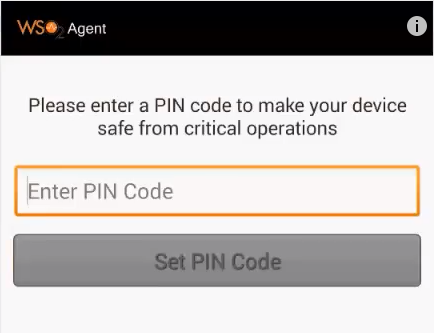
\includegraphics[scale=0.65]{res/EMM005}
\caption{Установка PIN-кода}
\end{figure}

\subsubsection{Возможности сервера}

После установки клиента, устройство появляется в списке всех устройств в веб-интерфейсе администратора. Администратор может видеть уникальный номер устройства, тип операционной системы (Android или iOS) и её версию, а так же пользователя этого устройства. Для простоты навигации, устройства можно группировать.

\begin{figure}[h!]
\centering
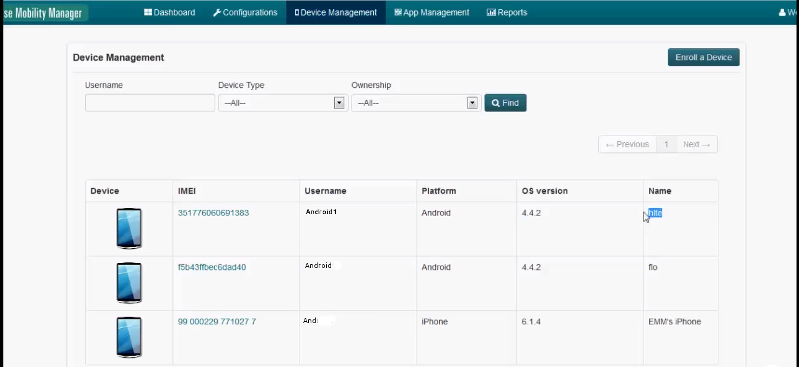
\includegraphics[scale=0.6]{res/EMM006}
\caption{Список устройств}
\end{figure}

Администратор получает достаточно широкие возможности управления мобильным телефоном, среди них:
\begin{itemize}
\item Блокирование звука (mute)
\item Политики паролей
\item Установка (сброс) паролей
\item Блокировка устройства
\item Управление подключениями (WiFi, Bluetooth)
\item Зашифрованное хранилище (только андроид!)
\item Отправка сообщений (владельцу телефона)
\item Полная очистка памяти телефона (к заводским настройкам)
\item Настройки почты
\item Управление камерой
\end{itemize}

Кроме того, администратор имеет лог последних операций, местоположение пользователя (его телефона) и может самостоятельно устанавливать и удалять приложения.

\section{WSO2 Developer Studio}

WSO2 Developer Studio представляет из себя Eclipse дополненный набором плагинов от WSO2. Установка среды разработки от WSO2 делается аналогично обычному Eclipse, нужно просто распаковать zip-архив..

Единственный важный момент о котором стоит помнить, это разнесение по портам различных продуктов WSO2 при их одновременном запуске. Для этой цели используется файла carbon.xml, а значения портов нужно прописать в теге <Offset>.

Подключение Enterprsie Mobility Manager к Developer Studio позволяет обеспечить запуск и просмотр логи сразу из среды программирования.

\begin{figure}[h!]
\centering
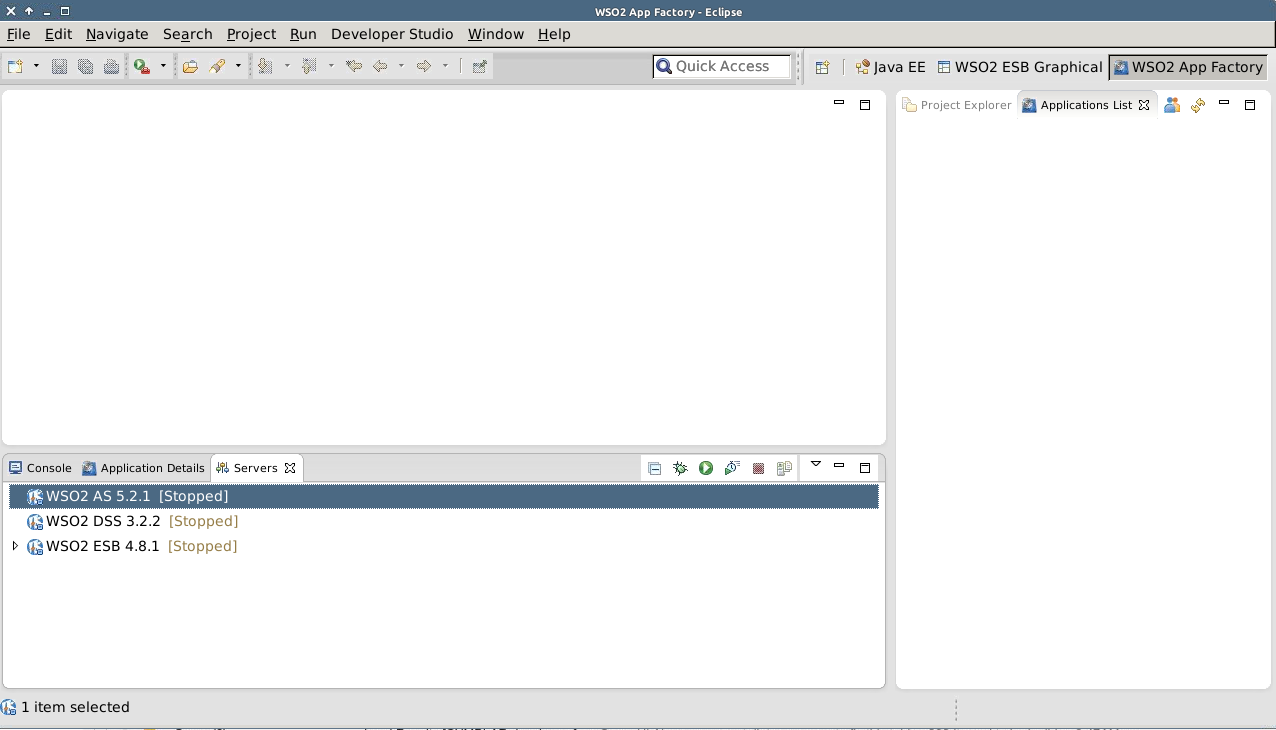
\includegraphics[scale=0.4]{res/DS001}
\caption{WSO2 Developer Studio}
\end{figure}

\section*{Заключение}
\addcontentsline{toc}{section}{Заключение}

Компания WSO2 представила целый ряд интересных продуктов. Некоторая часть  заявленного функционала работает не так, как заявленов описании, так что для решения о применимости этого решения требуется дополнительное изучение темы.

%------------------------------------------------------------------------------

\end{document}